\documentclass{llncs}
\usepackage{graphicx}
\usepackage[caption=false]{subfig}
\usepackage[dvipsnames]{xcolor}
\newcommand{\todo}[1]{\textcolor{red}{TODO: #1}}
\title{Old or Heavy?\\Decaying Gracefully with Age/Weight Shapes.}
\titlerunning{Dynamic Strategy Priority}
\authorrunning{Reger \and Rawson}
\author{Michael Rawson \and Giles Reger}
\institute{University of Manchester, Manchester, UK}

\begin{document}
\maketitle
\begin{abstract}
Vampire is an automatic theorem prover for first-order logic.
During proof search in given-clause algorithms, Vampire repeatedly selects clauses from either an \emph{age} or a \emph{weight} queue in a fixed, but configurable \emph{age/weight ratio} (AWR).
We show that an optimal fixed value of this ratio can produce proofs significantly more quickly on a given problem, and further that varying AWR during proof search can improve upon a fixed ratio.
Based on these observations we develop several new modes for Vampire which vary AWR according to a ``shape'' during proof search.
The modes solve a number of new problems in the TPTP benchmark.
\end{abstract}

\section{Introduction}
\label{sec:introduction}
\todo{standard Vampire~\cite{vampire} fluff here}.\\
\todo{explain a generic given-clause algorithm, define clause age and weight --- and how the ``balancing'' algorithm works internally}.\\
\todo{remark on portfolio modes --- more choice is (sometimes) a good thing}.

\section{Optimising Age/Weight Ratios}
\todo{talk about optimising for fixed age/weight}.\\
\todo{talk about experiments with changing age/weight}.

\section{Variable AWR for Vampire}
If changing AWR is sometimes useful for finding proofs more quickly, this could be useful as a Vampire option.
In general we would like to describe any possible sequence that the AWR could follow during proof search.
However, some details constrain the design space:
\begin{enumerate}
	\item Changing the AWR too frequently or sharply has little effect, due to the ``balancing'' algorithm --- see Section \ref{sec:introduction}.
	\item A general (configurable) \emph{shape} is more likely to be widely applicable than a specific series of data points.
	\item The shape must extend naturally to an indefinitely-long proof search.
\end{enumerate}

In this work we selected two general trends to explore: a trend away from the original (fixed) AWR toward 1:1 (``decay''), and a trend from 1:1 toward the original setting (``converge'').
Since a simple linear shape does not extend well to indefinite proof search (what should happen after either 1:1 or the target AWR is reached?), an exponential decay function is used instead, as shown in Figure \ref{fig:decay-and-converge}.

These shapes are further parameterised by an integral \emph{shape frequency} setting, which controls the rate of decay or convergence: every \(n\) steps, the difference between the current and the target AWR is halved, rounding where necessary.
In future, this might allow the use of repeating patterns such as a sinusoid, hence \emph{frequency}.

Our approach here was restricted by the balancing algorithm used internally, as AWR steps must be discrete and do not take effect immediately.
An alternative approach might use an age/weight probability, rather than a ratio, from which age or weight decisions would be pseudo-randomly (but reproducably) taken with the use of a seeded PRNG.
This would permit use of continuous age/weight functions, but would also introduce the possibility of ``getting unlucky'' in which a clause preferred by the age/weight probability is not selected due to an improbable-but-possible series of PRNG samples.

\begin{figure}
	\subfloat{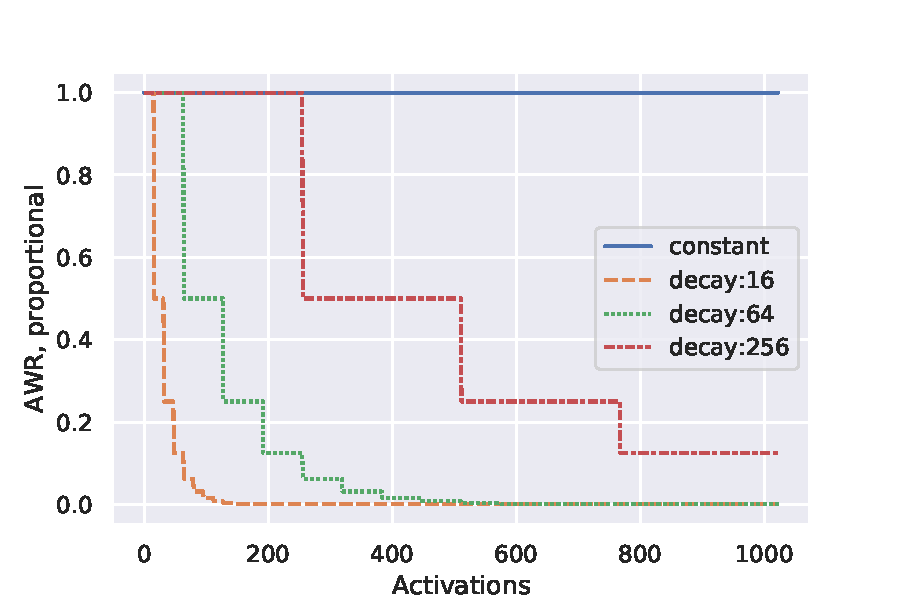
\includegraphics[width=0.5\textwidth]{shape-decay}}
	\subfloat{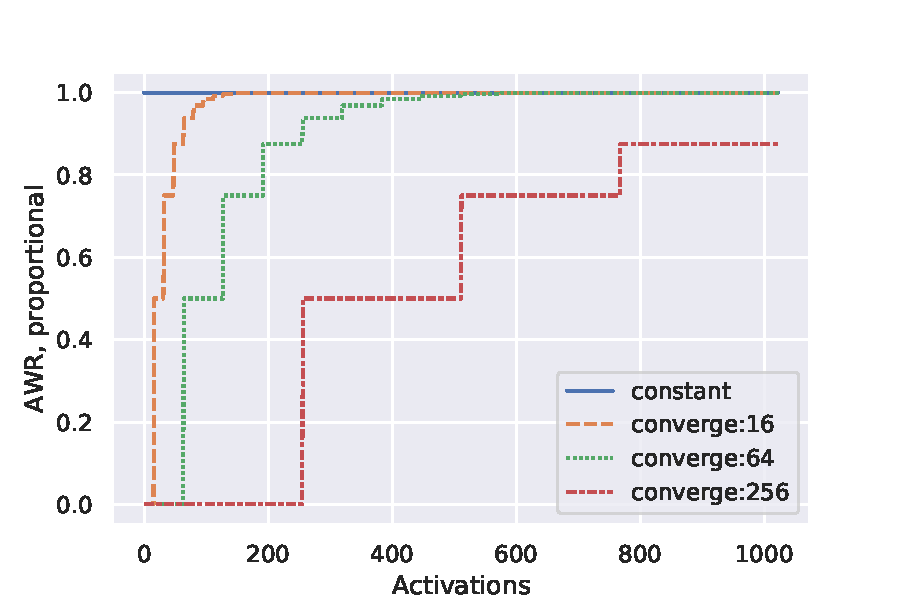
\includegraphics[width=0.5\textwidth]{shape-converge}}
	\caption{The new \emph{decay} and \emph{converge} AWR shapes as implemented in Vampire. Different curves exhibit the effect of the AWR shape frequency setting.}
	\label{fig:decay-and-converge}
\end{figure}

Together, these new settings allow a number of new option combinations, which can be used in conjunction with Vampire's portfolio \emph{CASC mode} pending integration into the strategy schedules.

\section{Experimental Evaluation}
In practice, decaying from an age-biased initial AWR to 1:1 (or converging backwards) was not found to be an improvement.
However, age/weight shapes starting with a weight-based AWR were found to be useful in some cases.
An experimental evaluation of this approach on the TPTP~\cite{tptp} benchmark follows.

\todo{analyse (two sets of) results, discuss drop in performance in exchange for uniques}.

\section{Future Work}
\todo{more shapes, better ways of doing frequency decay, integrate into existing strategy schedules}.

\section{Conclusions}
\todo{this is a thing, you can do it, you should do it (?), we can probably do better}.

\bibliographystyle{plain}
\bibliography{references}
\end{document}
